% Options for packages loaded elsewhere
\PassOptionsToPackage{unicode}{hyperref}
\PassOptionsToPackage{hyphens}{url}
\PassOptionsToPackage{dvipsnames,svgnames,x11names}{xcolor}
%
\documentclass[
  12pt,
  letterpaper,
]{report}

\usepackage{amsmath,amssymb}
\usepackage{setspace}
\usepackage{iftex}
\ifPDFTeX
  \usepackage[T1]{fontenc}
  \usepackage[utf8]{inputenc}
  \usepackage{textcomp} % provide euro and other symbols
\else % if luatex or xetex
  \usepackage{unicode-math}
  \defaultfontfeatures{Scale=MatchLowercase}
  \defaultfontfeatures[\rmfamily]{Ligatures=TeX,Scale=1}
\fi
\usepackage{lmodern}
\ifPDFTeX\else  
    % xetex/luatex font selection
  \setmainfont[]{Times New Roman}
  \setsansfont[]{Times New Roman}
\fi
% Use upquote if available, for straight quotes in verbatim environments
\IfFileExists{upquote.sty}{\usepackage{upquote}}{}
\IfFileExists{microtype.sty}{% use microtype if available
  \usepackage[]{microtype}
  \UseMicrotypeSet[protrusion]{basicmath} % disable protrusion for tt fonts
}{}
\usepackage{xcolor}
\setlength{\emergencystretch}{3em} % prevent overfull lines
\setcounter{secnumdepth}{5}
% Make \paragraph and \subparagraph free-standing
\ifx\paragraph\undefined\else
  \let\oldparagraph\paragraph
  \renewcommand{\paragraph}[1]{\oldparagraph{#1}\mbox{}}
\fi
\ifx\subparagraph\undefined\else
  \let\oldsubparagraph\subparagraph
  \renewcommand{\subparagraph}[1]{\oldsubparagraph{#1}\mbox{}}
\fi


\providecommand{\tightlist}{%
  \setlength{\itemsep}{0pt}\setlength{\parskip}{0pt}}\usepackage{longtable,booktabs,array}
\usepackage{calc} % for calculating minipage widths
% Correct order of tables after \paragraph or \subparagraph
\usepackage{etoolbox}
\makeatletter
\patchcmd\longtable{\par}{\if@noskipsec\mbox{}\fi\par}{}{}
\makeatother
% Allow footnotes in longtable head/foot
\IfFileExists{footnotehyper.sty}{\usepackage{footnotehyper}}{\usepackage{footnote}}
\makesavenoteenv{longtable}
\usepackage{graphicx}
\makeatletter
\def\maxwidth{\ifdim\Gin@nat@width>\linewidth\linewidth\else\Gin@nat@width\fi}
\def\maxheight{\ifdim\Gin@nat@height>\textheight\textheight\else\Gin@nat@height\fi}
\makeatother
% Scale images if necessary, so that they will not overflow the page
% margins by default, and it is still possible to overwrite the defaults
% using explicit options in \includegraphics[width, height, ...]{}
\setkeys{Gin}{width=\maxwidth,height=\maxheight,keepaspectratio}
% Set default figure placement to htbp
\makeatletter
\def\fps@figure{htbp}
\makeatother
\newlength{\cslhangindent}
\setlength{\cslhangindent}{1.5em}
\newlength{\csllabelwidth}
\setlength{\csllabelwidth}{3em}
\newlength{\cslentryspacingunit} % times entry-spacing
\setlength{\cslentryspacingunit}{\parskip}
\newenvironment{CSLReferences}[2] % #1 hanging-ident, #2 entry spacing
 {% don't indent paragraphs
  \setlength{\parindent}{0pt}
  % turn on hanging indent if param 1 is 1
  \ifodd #1
  \let\oldpar\par
  \def\par{\hangindent=\cslhangindent\oldpar}
  \fi
  % set entry spacing
  \setlength{\parskip}{#2\cslentryspacingunit}
 }%
 {}
\usepackage{calc}
\newcommand{\CSLBlock}[1]{#1\hfill\break}
\newcommand{\CSLLeftMargin}[1]{\parbox[t]{\csllabelwidth}{#1}}
\newcommand{\CSLRightInline}[1]{\parbox[t]{\linewidth - \csllabelwidth}{#1}\break}
\newcommand{\CSLIndent}[1]{\hspace{\cslhangindent}#1}

% page setup
\usepackage[letterpaper, margin=1in, footskip=0.5in]{geometry}
\special{papersize=8.5in,11in}

% fonts
\usepackage{fontspec}
\usepackage{setspace}
\newfontfamily\ko{Dotum}
\newfontfamily\zh{DengXian}
\newfontfamily\sy{Segoe UI Symbol}
\raggedright

% linguistic examples
\usepackage{expex}
\lingset{
  glhangstyle=none, 
  aboveglftskip=0pt, 
  everygla={},
  Everyex=\singlespace
  }
\usepackage{etoolbox}
\pretocmd{\chapter}{\excnt=1}{}{}

% syntactic trees
\usepackage{xytree}
\usepackage{textcomp}
\usepackage[linguistics]{forest}

% indentation
\usepackage{indentfirst}
\setlength{\parindent}{0.5in}

% captions
\usepackage[captionskip=0pt]{floatrow}
\floatsetup[figure]{capposition=top}
\floatsetup[table]{capposition=top}
\floatplacement{figure}{H}
\floatplacement{table}{H}
\usepackage[singlelinecheck=false, labelfont=bf, labelsep=newline, textfont=it, justification=raggedright, skip=0pt]{caption}

% enable 
\usepackage{graphicx}
\setlength\tabcolsep{3pt} % cell padding

% misc
\usepackage{multicol}
\usepackage{pdfpages}
\usepackage{contour}
%\usepackage{showframe} % show page margins

% reformat chapter headings
\makeatletter
\def\@makechapterhead#1{
  {\parindent \z@ \centering \normalfont \singlespacing
    \ifnum \c@secnumdepth >\m@ne
        \normalsize \bfseries \MakeUppercase \@chapapp\space \MakeUppercase{\thechapter}
        \par\nobreak
        \vskip 5\p@
    \fi
    \interlinepenalty\@M
    \normalsize \bfseries \MakeUppercase{#1}\par\nobreak
    \vskip 10\p@
  }}
\def\@makeschapterhead#1{
  {\parindent \z@ \centering
    \normalfont
    \interlinepenalty\@M
    \normalsize \bfseries \MakeUppercase{#1}\par\nobreak
    \vskip 10\p@
  }}
\makeatother

% reformat section headings
\makeatletter
\renewcommand{\section}{\@startsection{section}{1}{0pt}{0.5\baselineskip}{0.2\baselineskip}{\normalfont\normalsize\bfseries}}
\renewcommand{\subsection}{\@startsection{subsection}{2}{0pt}{0.5\baselineskip}{0.2\baselineskip}{\normalfont\normalsize\bfseries}}
\renewcommand{\subsubsection}{\@startsection{subsubsection}{3}{0pt}{0.5\baselineskip}{0.2\baselineskip}{\normalfont\normalsize\bfseries}}
\makeatother

% reformat table of contents, list of tables, and list of figures
\usepackage{titletoc}
\usepackage{tocloft}
\setlength{\cftbeforetoctitleskip}{0.8in}
\renewcommand{\cfttoctitlefont}{\normalfont\MakeUppercase\raggedright}
\renewcommand{\cftchapleader}{\cftdotfill{\cftdotsep}}
\renewcommand{\cftpartleader}{\cftdotfill{\cftdotsep}}
\titlecontents{part}
[0pt] % left margin
{\addvspace{1em}\bfseries\normalsize} % above code
{\MakeUppercase\partname~\thecontentslabel\hspace{1em}} % numbered entry format
{} % unnumbered entry format
{} % filler-page-format, e.g., dots
[\addvspace{0em}] % below code
\renewcommand{\cftfigfont}{\raggedright}
\renewcommand{\cfttabfont}{\raggedright}
\cftsetindents{figure}{0em}{2.5em}
\cftsetindents{table}{0em}{2.5em}

% include part titles in the toc but hide them in the body
\renewcommand{\part}[1]{\addcontentsline{toc}{part}{#1}}

% define commands for adding colored boxes around text
\usepackage{tikz}
\newcommand{\add}[2][]{%
  \begin{tikzpicture}[baseline = (text.base)]%
    \node[%
      inner sep = 2pt,
      text depth = depth("Cap") + 1pt,
      text height = height("Cap") + 1pt,
      fill=green!20!white,
      draw=green!80!black,
      solid,
      line width=0.6pt,
      sharp corners,
  #1] (text) {#2};
  \end{tikzpicture}%
}%
\newcommand{\remove}[2][]{%
  \begin{tikzpicture}[baseline = (text.base)]%
    \node[%
      inner sep = 2pt,
      text depth = depth("Cap") + 1pt,
      text height = height("Cap") + 1pt,
      fill=red!20!white,
      draw=red,
      dashed,
      line width=0.6pt,
      sharp corners,
  #1] (text) {#2};
  \end{tikzpicture}%
}%
\newcommand{\gap}[2][]{%
  \begin{tikzpicture}[baseline = (text.base)]%
    \node[%
      inner sep = 2pt,
      text depth = depth("Cap") + 1pt,
      text height = height("Cap") + 1pt,
      draw=black,
      solid,
      text width=5em,
      align = center,
      line width=0.6pt,
      sharp corners,
  #1] (text) {#2};
  \end{tikzpicture}%
}%
\usepackage{booktabs}
\usepackage{longtable}
\usepackage{array}
\usepackage{multirow}
\usepackage{wrapfig}
\usepackage{float}
\usepackage{colortbl}
\usepackage{pdflscape}
\usepackage{tabu}
\usepackage{threeparttable}
\usepackage{threeparttablex}
\usepackage[normalem]{ulem}
\usepackage{makecell}
\usepackage{xcolor}
\usepackage{expex}
\let\expexgla\gla
\AtBeginDocument{\let\gla\expexgla}
\makeatletter
\makeatother
\makeatletter
\@ifpackageloaded{bookmark}{}{\usepackage{bookmark}}
\makeatother
\makeatletter
\@ifpackageloaded{caption}{}{\usepackage{caption}}
\AtBeginDocument{%
\ifdefined\contentsname
  \renewcommand*\contentsname{Table of contents}
\else
  \newcommand\contentsname{Table of contents}
\fi
\ifdefined\listfigurename
  \renewcommand*\listfigurename{}
\else
  \newcommand\listfigurename{}
\fi
\ifdefined\listtablename
  \renewcommand*\listtablename{}
\else
  \newcommand\listtablename{}
\fi
\ifdefined\figurename
  \renewcommand*\figurename{Figure}
\else
  \newcommand\figurename{Figure}
\fi
\ifdefined\tablename
  \renewcommand*\tablename{Table}
\else
  \newcommand\tablename{Table}
\fi
}
\@ifpackageloaded{float}{}{\usepackage{float}}
\floatstyle{ruled}
\@ifundefined{c@chapter}{\newfloat{codelisting}{h}{lop}}{\newfloat{codelisting}{h}{lop}[chapter]}
\floatname{codelisting}{Listing}
\newcommand*\listoflistings{\listof{codelisting}{List of Listings}}
\makeatother
\makeatletter
\@ifpackageloaded{caption}{}{\usepackage{caption}}
\@ifpackageloaded{subcaption}{}{\usepackage{subcaption}}
\makeatother
\makeatletter
\@ifpackageloaded{tcolorbox}{}{\usepackage[skins,breakable]{tcolorbox}}
\makeatother
\makeatletter
\@ifundefined{shadecolor}{\definecolor{shadecolor}{rgb}{.97, .97, .97}}
\makeatother
\makeatletter
\makeatother
\makeatletter
\makeatother
\ifLuaTeX
  \usepackage{selnolig}  % disable illegal ligatures
\fi
\IfFileExists{bookmark.sty}{\usepackage{bookmark}}{\usepackage{hyperref}}
\IfFileExists{xurl.sty}{\usepackage{xurl}}{} % add URL line breaks if available
\urlstyle{same} % disable monospaced font for URLs
\hypersetup{
  colorlinks=true,
  linkcolor={black},
  filecolor={Maroon},
  citecolor={Blue},
  urlcolor={Blue},
  pdfcreator={LaTeX via pandoc}}

\author{}
\date{}

\begin{document}
\pagenumbering{gobble}

\begin{centering}

\vspace{3cm}

\doublespacing
DISSERTATION TITLE

\vspace{1.5cm}

\singlespacing
A DISSERTATION SUBMITTED TO THE GRADUATE DIVISION OF \\
UNIVERSITY NAME IN PARTIAL FULFILLMENT OF \\
THE REQUIREMENTS FOR THE DEGREE OF

\vspace{1cm}

\doublespacing
DOCTOR OF PHILOSOPHY \\
IN \\
DEPARTMENT NAME

\vspace{1.5cm}

\singlespacing
SEPTEMBER 2023

\vspace{1.5cm}

\doublespacing
By \\
Author Name

\vspace{1.5 cm}

\singlespacing
Dissertation Committee: \\
First Person, Chairperson \\
Second Person \\
Third Person \\
Fourth Person \\
Fifth Person

\vspace*{\fill}

\flushleft
Keywords: first keyword, second keyword, third keyword

\end{centering}

\newpage

\pagenumbering{roman}

\setcounter{page}{1}

\vspace*{\fill}

\begin{centering}

Copyright \textcopyright \space 2023

\vspace{0.5 cm}

Author Name

All Rights Reserved

\end{centering}

\newpage

\begin{spacing}{1.5}

\chapter*{Acknowledgments}
\addcontentsline{toc}{chapter}{Acknowledgments}

\newpage

\chapter*{Abstract}
\addcontentsline{toc}{chapter}{Abstract}

\end{spacing}

\newpage

\ifdefined\Shaded\renewenvironment{Shaded}{\begin{tcolorbox}[enhanced, frame hidden, breakable, boxrule=0pt, borderline west={3pt}{0pt}{shadecolor}, sharp corners, interior hidden]}{\end{tcolorbox}}\fi

\renewcommand*\contentsname{\vspace{-3cm} \begin{center} \normalsize \textbf{TABLE OF CONTENTS} \end{center} \vspace{-1.5cm}}
{
\hypersetup{linkcolor=}
\setcounter{tocdepth}{2}
\tableofcontents
}
\setstretch{1.5}
\bookmarksetup{startatroot}

\hypertarget{list-of-tables}{%
\chapter*{List of Tables}\label{list-of-tables}}
\addcontentsline{toc}{chapter}{List of Tables}

\markboth{List of Tables}{List of Tables}

\vspace{-3 cm}

\listoftables

\newpage

\bookmarksetup{startatroot}

\hypertarget{list-of-figures}{%
\chapter*{List of Figures}\label{list-of-figures}}
\addcontentsline{toc}{chapter}{List of Figures}

\markboth{List of Figures}{List of Figures}

\vspace{-3 cm}

\listoffigures

\bookmarksetup{startatroot}

\hypertarget{list-of-abbreviations}{%
\chapter*{List of Abbreviations}\label{list-of-abbreviations}}
\addcontentsline{toc}{chapter}{List of Abbreviations}

\markboth{List of Abbreviations}{List of Abbreviations}

\renewcommand\thepage{\romannumeral\numexpr\value{page}\relax}

\part{Chapters}

\hypertarget{a-chapter-with-some-text}{%
\chapter{A Chapter With Some Text}\label{a-chapter-with-some-text}}

\pagenumbering{arabic}
\setcounter{page}{1}

Lorem ipsum dolor sit amet, consectetur adipiscing elit. Cras a lectus
aliquet, placerat massa id, vestibulum nisl. Aliquam pellentesque quis
nibh sed tempus. Proin luctus ultrices erat, mollis volutpat enim
pellentesque eu. Ut tellus orci, rhoncus egestas porta sagittis,
eleifend id libero. Fusce pretium interdum condimentum. Aenean malesuada
volutpat cursus. Maecenas eget felis diam. Donec congue, erat sit amet
pretium egestas, massa dolor vehicula odio, vel pharetra mi diam eget
ipsum. Vivamus massa felis, commodo et metus eu, vehicula elementum
eros. Donec et rutrum justo. Morbi dignissim est a sapien commodo
bibendum. Nulla sit amet fermentum enim. Integer interdum lobortis eros.
Fusce nec ultrices mauris. Maecenas eget ullamcorper orci. Nulla
vestibulum lobortis tortor et sollicitudin.

Quisque egestas laoreet leo, quis commodo velit congue nec. Proin vitae
turpis lobortis, porttitor enim tincidunt, ultrices orci. Nam nulla
nisi, imperdiet nec tincidunt at, hendrerit non eros. In pharetra
hendrerit justo non rutrum. Suspendisse potenti. Integer ac eros quis
lacus porttitor efficitur. Sed fermentum libero vel mauris vulputate, et
cursus velit semper. Curabitur aliquam, augue vitae vulputate consequat,
sem enim aliquam quam, nec sodales lacus purus quis nibh. Nulla
faucibus, quam quis porta rutrum, ante orci congue nisi, vel tristique
est ipsum vel dui. Class aptent taciti sociosqu ad litora torquent per
conubia nostra, per inceptos himenaeos.

Mauris consequat scelerisque justo quis fermentum. Aliquam ac tempor
ante, facilisis faucibus tellus. Fusce et urna non eros scelerisque
aliquet sit amet sed dolor. Suspendisse a cursus nisl. Suspendisse
vehicula sagittis elit, eget hendrerit erat imperdiet sed. Aenean dictum
sed urna at maximus. Nunc varius quis elit in euismod. Nunc tincidunt ut
nisi vel mattis. Suspendisse sed sagittis ex. Integer convallis eget
nisi sit amet tincidunt. Integer aliquet, odio non iaculis auctor, mi
ligula interdum neque, ullamcorper blandit metus metus id ex.

\hypertarget{a-chapter-with-a-table}{%
\chapter{A Chapter With a Table}\label{a-chapter-with-a-table}}

See Table~\ref{tbl-example} below.

\begin{table}

\caption{\label{tbl-example}Example
Table}\begin{minipage}[t]{\linewidth}

{\centering 

\hypertarget{tbl-example-1}{}
\begin{tabu} to \linewidth {>{\raggedleft}X>{\raggedleft}X>{\raggedleft}X>{\raggedleft}X>{\raggedright}X}
\toprule
Sepal.Length & Sepal.Width & Petal.Length & Petal.Width & Species\\
\midrule
5.1 & 3.5 & 1.4 & 0.2 & setosa\\
4.9 & 3.0 & 1.4 & 0.2 & setosa\\
4.7 & 3.2 & 1.3 & 0.2 & setosa\\
4.6 & 3.1 & 1.5 & 0.2 & setosa\\
5.0 & 3.6 & 1.4 & 0.2 & setosa\\
\addlinespace
5.4 & 3.9 & 1.7 & 0.4 & setosa\\
\bottomrule
\end{tabu}

}

\end{minipage}%
\newline
\begin{minipage}[t]{\linewidth}

{\centering 

\flushleft\textit{Note}. Table note.

}

\end{minipage}%

\end{table}

\hypertarget{a-chapter-with-a-figure}{%
\chapter{A Chapter With a Figure}\label{a-chapter-with-a-figure}}

See Figure~\ref{fig-example} below.

\begin{figure}

{\centering 

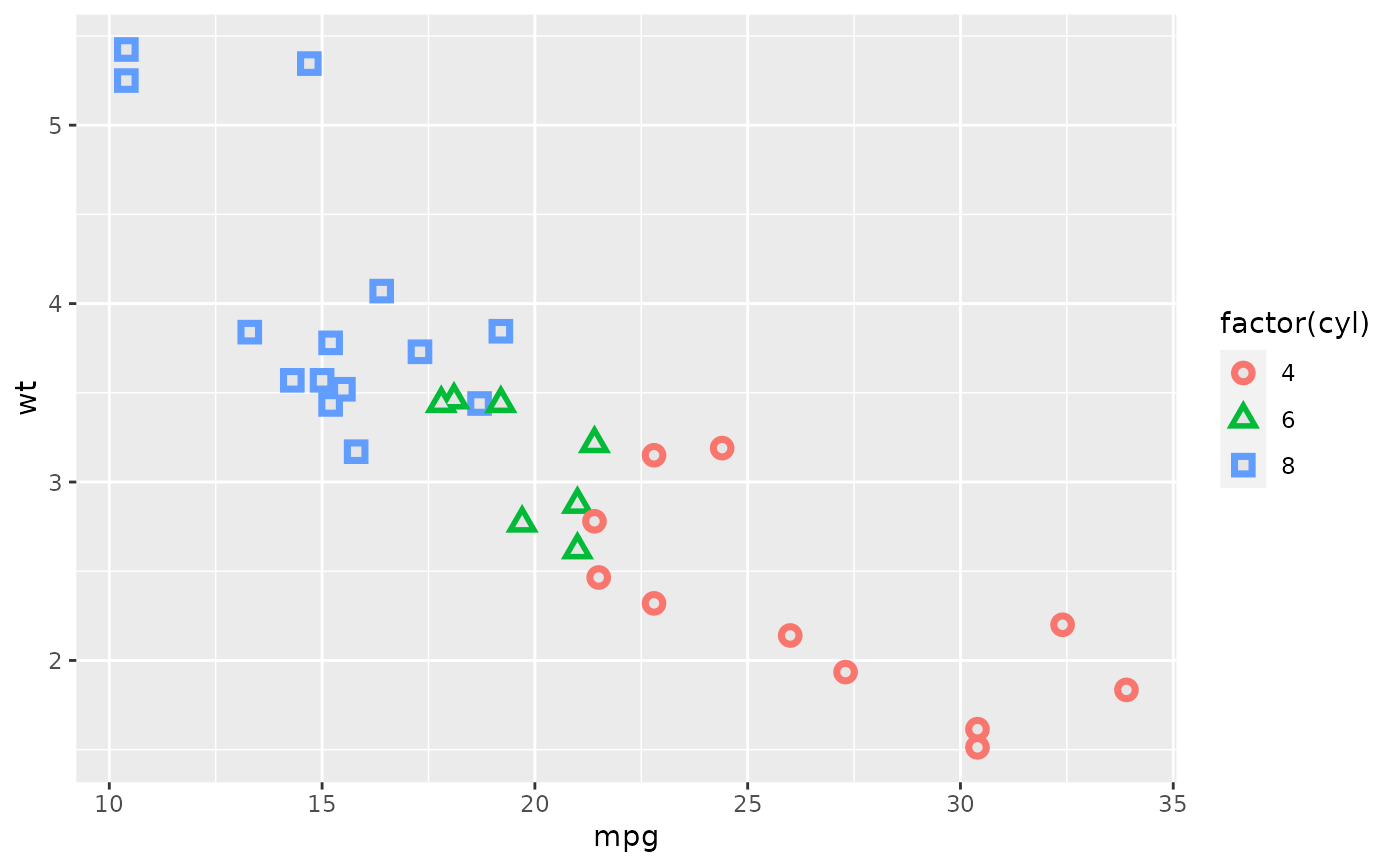
\includegraphics{image/example.png}

\hypertarget{fig-example-1}{}
\raggedright

\textit{Note}. Figure Note.

}

\caption{\label{fig-example}Example Figure}

\end{figure}

\hypertarget{a-chapter-with-a-syntactic-tree}{%
\chapter{A Chapter With a Syntactic
Tree}\label{a-chapter-with-a-syntactic-tree}}

See (\ref{tree-break}) below.

\ex \label{tree-break}
\begin{forest}
    for tree = {parent anchor = south, child anchor = north}
    [NP 
        [Det 
            [the]
        ] 
        [N$'$ 
            [N 
                [boy]
            ] 
            [CP 
                [NP 
                    [N 
                        [who, name = target]
                    ] 
                ]
                [C$'$ 
                    [C 
                        [+Rel]
                    ] 
                    [TP 
                        [NP 
                            [\textit{t}, name = source]
                        ] 
                        [T$'$ 
                            [T 
                                [+PST]
                            ]
                            [VP 
                                [V 
                                    [broke]
                                ] 
                                [NP 
                                    [the window, roof ]
                                ]
                            ]
                        ]
                    ]
                ]
            ]
        ]
    ]
    \draw[->] (source) to [out=south, in=south] (target);
\end{forest}
\xe

\hypertarget{a-chapter-with-some-linguistic-glosses}{%
\chapter{A Chapter With Some Linguistic
Glosses}\label{a-chapter-with-some-linguistic-glosses}}

See (\ref{ex-kor}) below.

\lingset{exskip=0pt,belowglpreambleskip=0pt,aboveglftskip=0pt,extraglskip=0pt,everyglpreamble=,everygla=,everyglb=,everyglc=,everyglft=}

\ex \begingl \gla el libro que compré// \glb the book that buy.PST.1S//
\glft ``the book that I bought''// \endgl \xe

\pex[everygla=\ko] \label{ex-kor}
Example Relative Clauses in Korean
\a 
\begingl
\glpreamble \textit{First Example} //
\gla 내가 산 책 // 
\glb nay-ka sa-n chayk //
\glc {\sc 1s-nom} buy-{\sc rel} book //
\glft “the book that I bought” // 
\endgl 
\a 
\begingl
\glpreamble \textit{Second Example} //
\gla 내가 본 영화  // 
\glb nay-ka po-n yenghwa //
\glc {\sc 1s-nom} watch-{\sc rel} movie //
\glft “the movie that I watched” // 
\endgl 
\a 
\begingl
\glpreamble \textit{Third Example} //
\gla 당신을 좋아하는 사람 // 
\glb tangsin-ul cohaha-nun salam  //
\glc {\sc 2s-acc} like-{\sc rel} person //
\glft “the person who likes you” //
\endgl 
\xe

\pex[everygla=\zh]
Example Relative Clauses in Mandarin
\a 
\begingl
\glpreamble \textit{First Example} //
\gla 我 买 的 书 // 
\glb wo mai de shu //
\glc {\sc 1s-nom} buy {\sc rel} book //
\glft “the book that I bought” // 
\endgl 
\a 
\begingl
\glpreamble \textit{Second Example} //
\gla 我 看 过 的 电影  // 
\glb wo kan guo de dianying //
\glc {\sc 1s} watch {\sc asp} {\sc rel} movie //
\glft “the movie that I watched” // 
\endgl 
\a 
\begingl
\glpreamble \textit{Third Example} //
\gla 喜欢 你 的 人 // 
\glb xihuan ni de ren  //
\glc like {\sc 2s} {\sc rel} person //
\glft “the person who likes you” //
\endgl 
\xe

\hypertarget{a-chapter-with-some-citations}{%
\chapter{A Chapter With Some
Citations}\label{a-chapter-with-some-citations}}

This is a sentence with a parenthetical citation
(\protect\hyperlink{ref-smit54}{Smith \& Weston, 1954}; see also
\protect\hyperlink{ref-gree00}{Green et al., 1900};
\protect\hyperlink{ref-jame76}{James et al., 1776}). This is a sentence
with a text citation of Phillips (\protect\hyperlink{ref-phil99}{1999}).

\cleardoublepage
\phantomsection
\addcontentsline{toc}{part}{Appendices}
\appendix

\hypertarget{first-appendix}{%
\chapter{First Appendix}\label{first-appendix}}

\setlength{\parindent}{0in}
\singlespacing

\hypertarget{second-appendix}{%
\chapter{Second Appendix}\label{second-appendix}}

\hypertarget{third-appendix}{%
\chapter{Third Appendix}\label{third-appendix}}

\hypertarget{references}{%
\chapter*{References}\label{references}}
\addcontentsline{toc}{chapter}{References}

\markboth{References}{References}

\onehalfspacing

\hypertarget{refs}{}
\begin{CSLReferences}{1}{0}
\leavevmode\vadjust pre{\hypertarget{ref-gree00}{}}%
Green, R. J., Fred, U. P., \& Norbert, W. P. (1900). Things that go bump
in the night. \emph{Psych. Today}, \emph{46}, 345--678.

\leavevmode\vadjust pre{\hypertarget{ref-jame76}{}}%
James, K., Harris, G., Jr., \& Wollops, W. (1776). {American}
independence and magnetism. \emph{Revol. Tracts}, \emph{32}, 34--55.

\leavevmode\vadjust pre{\hypertarget{ref-phil99}{}}%
Phillips, T. P. (1999). Possible influence of the magnetosphere on
{American} history. \emph{J. Oddball Res.}, \emph{98}, 1000--1003.

\leavevmode\vadjust pre{\hypertarget{ref-smit54}{}}%
Smith, J. G., \& Weston, H. K. (1954). Nothing particular in this year's
history. \emph{J. Geophys. Res.}, \emph{2}, 14--15.

\end{CSLReferences}



\end{document}
